\documentclass[a4paper,11pt,twoside,openright]{book}

\usepackage{makeidx}
\usepackage{amsmath}
\usepackage{amssymb}
\usepackage{amsthm}
\usepackage{graphicx}
\usepackage{longtable}
\usepackage{lscape}
% change "blue" to "black" if printted
\usepackage[dvipdfm,draft=false,colorlinks=true,bookmarksnumbered=true,
            hyperindex,pdfstartview=FitH,plainpages=false,
            linkcolor=blue,citecolor=blue,urlcolor=blue]{hyperref}
%CJKbookmarks=true
\usepackage[square,comma,numbers,sort&compress]{natbib}
\usepackage{hypernat}
%\usepackage{citesort}  %sort citations
\usepackage[T1]{fontenc} %make nice pdf on screen

\usepackage{tikz}
\usetikzlibrary{shapes,arrows,shapes.geometric,calc}

% all the figures are in directory "figures"
\graphicspath{{figures/}}

% footnote style
\renewcommand{\thefootnote}{\fnsymbol{footnote}}

% used for notice, remove this at the end
\usepackage{xcolor}
\newcommand{\fixme}[1]{\textbf{\textit{\color{red} #1}}}

% page layout
\setlength{\marginparwidth}{0in}
\setlength{\evensidemargin}{-0.4in}
\setlength{\oddsidemargin}{-0.07in} 
\setlength{\textwidth}{6.76in}
\setlength{\topmargin}{0in}
\setlength{\textheight}{9in}

% define block styles
\tikzstyle{module} = [rectangle, draw, text width=2cm, text centered, sharp corners, %
minimum height=1cm, node distance=4cm]
\tikzstyle{arrow} = [draw, very thick, -latex']

\begin{document}

% front matter
\frontmatter
\pagestyle{empty}

% title page
\vspace*{\fill}
\begin{center}
  \begin{Huge}\textsf{OpenR{\huge SP} Manual}\end{Huge}\\[0.5\baselineskip]
  \begin{LARGE}\textsf{Version 0.1.0}\end{LARGE}
\end{center}

\vspace*{\fill}
\begin{center}
  \begin{huge}\textsf{Authors}\end{huge}\\[0.5\baselineskip]
  \begin{LARGE}\textsf{\today}\end{LARGE}
\end{center}

\vspace*{\fill}
\begin{center}
  \begin{large}
    \textsf{Centre for Theoretical and Computational Chemistry (CTCC)}\par
    \textsf{Department of Chemistry}\par
    \textsf{University of Troms{\o}, N--9037}\par
    \textsf{Troms{\o}, Norway}\\[0.5\baselineskip]
  \end{large}
\end{center}

\clearpage

% copyright page
\begingroup
\footnotesize
\setlength{\parindent}{0pt}
\setlength{\parskip}{\baselineskip}
\textcopyright{} 2009~--~2011 Authors\\

Open\textsc{Rsp} is free software: you can redistribute it and/or modify
it under the terms of the GNU Lesser General Public License as published by
the Free Software Foundation, either version 3 of the License, or
(at your option) any later version.

Open\textsc{Rsp} is distributed in the hope that it will be useful,
but WITHOUT ANY WARRANTY; without even the implied warranty of
MERCHANTABILITY or FITNESS FOR A PARTICULAR PURPOSE. See the
GNU Lesser General Public License for more details.

You should have received a copy of the GNU Lesser General Public License
along with Open\textsc{Rsp}. If not, see\linebreak \url{http://www.gnu.org/licenses/}.
\endgroup
\clearpage

% contents
\pagestyle{headings}

%\makeindex

\tableofcontents

% preface
\chapter*{Preface}
\label{chap:preface}

\addcontentsline{toc}{chapter}{Preface}

Open\textsc{Rsp} is 

% acknowledgments
\chapter*{Acknowledgments}
\label{chap:acknowledgments}

\addcontentsline{toc}{chapter}{Acknowledgments}

% body
\mainmatter
\pagenumbering{arabic}

% chapter of framework of OpenRsp
\chapter{Framework of Open\textsc{Rsp}}
\label{chap:framework}

\begin{figure}[htbp]
  \centering
  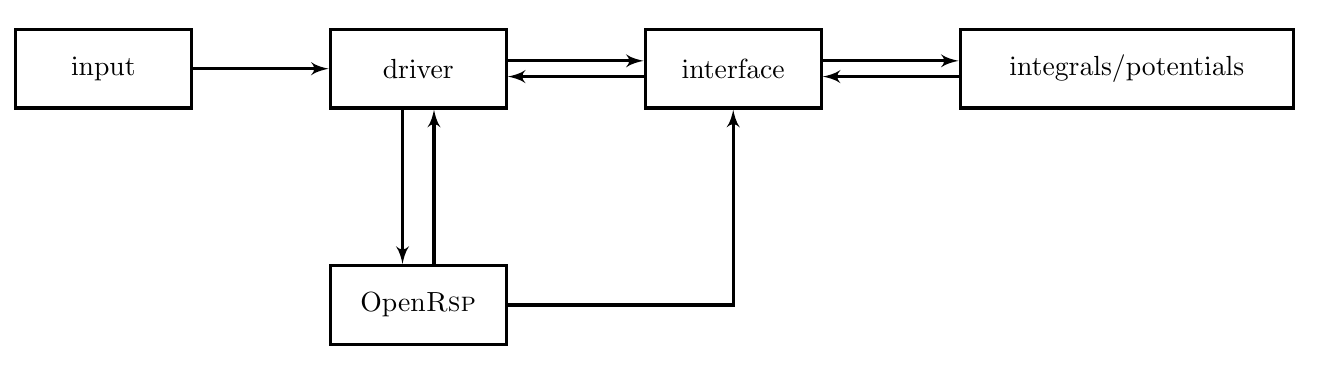
\begin{tikzpicture}[scale=1, style=very thick, auto]
    \node[module] (input) {input};
    \node[module, right of=input] (driver) {driver};
    \node[module, below of=driver, node distance=3cm] (openrsp) {Open\textsc{Rsp}};
    \node[module, right of=driver] (interface) {interface};
    \node[module, text width=4cm, right of=interface, node distance=5cm] (integrals) {integrals/potentials};
    % draw arrows
    \path[arrow] (input) -- (driver);
    \path[arrow] ($(driver.south)-(2mm,0)$) -- ($(openrsp.north)-(2mm,0)$);
    \path[arrow] ($(openrsp.north)+(2mm,0)$) -- ($(driver.south)+(2mm,0)$);
    \path[arrow] ($(driver.east)+(0,1mm)$) -- ($(interface.west)+(0,1mm)$);
    \path[arrow] ($(interface.west)-(0,1mm)$) -- ($(driver.east)-(0,1mm)$);
    \path[arrow] (openrsp) -| node [near start] {} (interface);
    \path[arrow] ($(interface.east)+(0,1mm)$) -- ($(integrals.west)+(0,1mm)$);
    \path[arrow] ($(integrals.west)-(0,1mm)$) -- ($(interface.east)-(0,1mm)$);
  \end{tikzpicture}
  \caption{Framework of Open\textsc{Rsp}.}
\end{figure}


% installation
\chapter{Installation}
\label{chap:installation}

% limitations
\chapter{Limitations}
\label{chap:limitations}

% back end
\backmatter

% references
\begin{small}
  \bibliographystyle{unsrt}
%  \bibliographystyle{abbrv}
  \bibliography{refs}
\end{small}

% index
%\part{Index}
%\printindex

\end{document}

